%parent:"exm:heegaardDiagram3Sphere"
%label:"fig:heegaardDiagram3Sphere"
%author:JeffHicks
%name:"Heegaard diagram for $S^3$"
%type:"figure"
%caption:"A Heegaard diagram for $S^3$. The attaching cycles $\alpha, \beta$ are drawn in red in the torus. The disks in red and blue represent the downward and upward flow spaces of the critical points $p, q$."


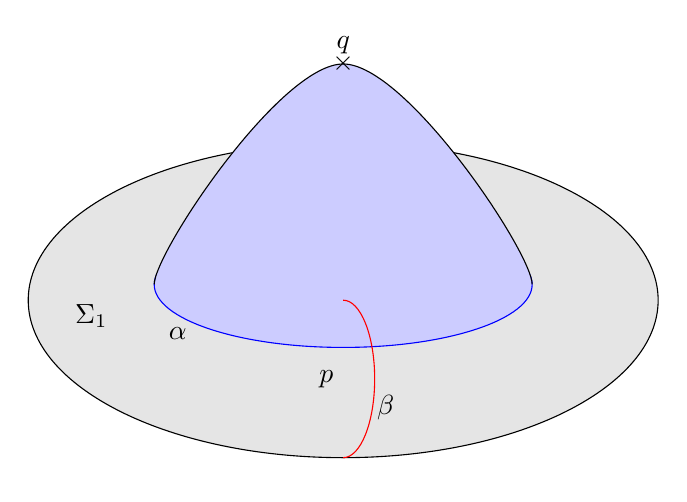
\begin{tikzpicture}[scale=2]

    \begin{scope}[]
    \clip  (-1.8,-1.6) rectangle (0,-0.2);
    \draw  (-1.2,-1) ellipse (0.2 and 0.5);
    \end{scope}
    
    
    \fill[red!20]  (-1.2,-1) ellipse (0.2 and 0.5);
    \node[] at (-1.2,-1) {$\times$};
    \draw[fill=gray!20,  fill opacity=95]  (-1.2,-0.5) ellipse (2 and 1);
    
     \begin{scope}[shift={(2.2,-0.6)}]
        
        \fill[white]  plot[smooth, tension=0.7] coordinates { (-3.68,0.2) (-3.4,0.1) (-3.14,0.2) }  plot[smooth, tension=0.7] coordinates {(-3.68,0.2) (-3.4,0.34) (-3.14,0.2)};
        
        \draw  plot[smooth, tension=0.7] coordinates {(-3.8,0.34) (-3.68,0.2) (-3.4,0.1) (-3.14,0.2) (-3,0.34)};
        \draw  plot[smooth, tension=0.7] coordinates {(-3.68,0.2) (-3.4,0.34) (-3.14,0.2)};
        
        
        
        \end{scope}
        
        
    \draw[draw=blue, fill=blue!20, fill opacity=90]  (-1.2,-0.4) node (v1) {} ellipse (1.2 and 0.4);
    
    \fill[fill=blue!20, fill opacity=90] (-2.4,-0.4) .. controls (-2.4,-0.2) and (-1.6,1) .. (-1.2,1) .. controls (-0.8,1) and (0,-0.2) .. (0,-0.4) .. controls (0,-0.2) and (-0.8,-0.2) .. (-1.2,-0.2) .. controls (-1.6,-0.2) and (-2.4,-0.2) .. (-2.4,-0.4);
    
    \draw (-2.4,-0.4) .. controls (-2.4,-0.2) and (-1.6,1) .. (-1.2,1) .. controls (-0.8,1) and (0,-0.2) .. (0,-0.4);
    
    \begin{scope}[]
    \clip  (-0.8,-1.6) rectangle (v1);
    \draw[red]  (-1.2,-1) ellipse (0.2 and 0.5);
    \end{scope}
    
    
    \node[left] at (-1.2,-1) {$p$};
    \node[above] at (-1.2,1) {$q$};
    \node at (-1.2,1) {$\times$};
    \node at (-2.25,-0.71) {$\alpha$};
    \node at (-0.93,-1.18) {$\beta$};
    \node at (-2.8,-0.6) {$\Sigma_1$};
    \end{tikzpicture}